\documentclass{../../ece-report}

\graphicspath{ {./imgs} }
\memostudent{Ty Davis}
\memotitle{Lab 1 - The Diode}
\memocourse{ECE 3110}
\memodate{\today}

\begin{document}

\maketitle
\section{Introduction}

In this lab we build a simple circuit utilizing a diode
and a resistor to measure and analyze the performance
of the diode under different condiditions. Before we
take measurements of the circuit, we solve for the voltages
and current through the circuit in a few different ways
and then compare our results. We will test our circuit
with a few different voltages to see how the components
respond.

\begin{figure}[h!]
  \centering
  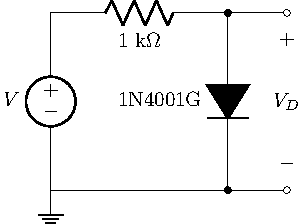
\includegraphics{../circuits/circuit1.pdf}
  \label{fig:circuit}
  \caption{The circuit we used in the lab.}
\end{figure}


\section{Theory}

To analyze the circuit we will make use of three ways
to model a diode, known as the \emph{ideal model}, \emph{constant
drop model}, and the \emph{exponential model}. For each
model we will calculate the current through the circuit,
and the voltages present around the resistor and the
diode for 10~V, 1.2~V, and 0.75~V (a voltage where we
found the current to drop off significantly).

\subsection{Ideal Model}

In the ideal model we assume that a diode is simply
a short circuit when forward biased, which leaves us
with a circuit as shown in Fig.~\ref{fig:ideal}.

\begin{figure}[h!]
  \centering
  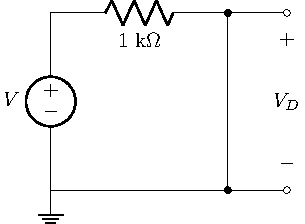
\includegraphics{../circuits/circuit_ideal.pdf}
  \label{fig:ideal}
  \caption{The circuit when using the ideal model.}
\end{figure}

Without a diode present, the current through the circuit is shown
with $I = \frac{V}{R}$, and the voltage over the diode is always 0~V.

For 10~V: $I=\frac{10~\si{\V}}{1~\si{\kohm}} = 10~\si{\mA}$ \\
For 1.2~V: $I=\frac{1.2~\si{\V}}{1~\si{\kohm}} = 1.2~\si{\mA}$ \\
For 0.75~V: $I=\frac{0.75~\si{\V}}{1~\si{\kohm}} = 0.75~\si{\mA}$


\subsection{Constant Drop}

The constant drop model for a diode suggests that a diode
can be replaced by a voltage source equalling 0.7~V with the positive
terminal aligned with the cathode of the diode. See Fig.~\ref{fig:constant}

\begin{figure}[h~]
  \centering
  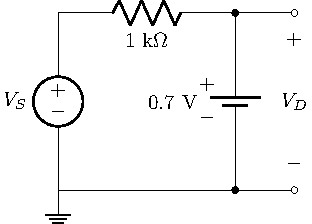
\includegraphics{../circuits/circuit_constant.pdf}
  \label{fig:constant}
  \caption{The circuit when usint the constant drop model.}
\end{figure}

With a supposed battery supplying voltage to the circuit,
the resulting voltage over that resistor is then reduced
to $V - 0.7~\si{\V}$. This means that the current through the circuit
is shown by $I = \frac{V - 0.7~\si{\V}}{R}$.

For 10~V: $I=\frac{9.3~\si{\V}}{1~\si{\kohm}} = 9.3~\si{\mA}$ \\
For 1.2~V: $I=\frac{0.6~\si{\V}}{1~\si{\kohm}} = 0.6~\si{\mA}$ \\
For 0.75~V: $I=\frac{0.15~\si{\V}}{1~\si{\kohm}} = 0.15~\si{\mA}$

\subsection{Exponential Model}

When using the exponential model, we use Eq.~\ref{eq:exponential}
to show the relationship between the current and the
voltage through a diode.

\begin{equation}
  \label{eq:exponential}
  I = I_S e ^ {V / V_{TH}}
\end{equation}

We are using a value of $V_{TH}=25.9~\si{\mV}$ for the
thermal voltage. $I_S$ is calculated by using an operating
point given from a datasheet in Eq.~\ref{eq:exponential}.
Rearranging the equation yields the following:

\[
  I_S = \frac{I}{e^{V/V_{TH}}}
\]

Plugging in our values we find:

\[
  I_S = \frac{1~\si{\A}}{e^{0.93~\si{\V}/25.9~\si{\mV}}} = \SI{2.545E-16}~\si{\A}
\]

Now, with a satisfactory $I_S$ value we can use the
iterative method to solve for the current and voltage
in the diode. Using the following two equations we can iterate on the values
of $I$ and $V_D$ until we have sufficiently accurate values.

\[
  
\]

\section{Graphical Analysis}

\section{Results}

\section{Conclusion}

\section{Extra Thoughts}


\end{document}
